% En las siguientes 3 paginas, debe incluir una digitalización de calidad de sus respectivas cartaas, no una fotografia toda cucha tomada con su celular de Coppel
% Pagina 1: Digitalización de la carta de presentación (sustituir por una original en el empastado)
\clearpage
\thispagestyle{fancy}
\pagenumbering{roman}
\setcounter{page}{1}
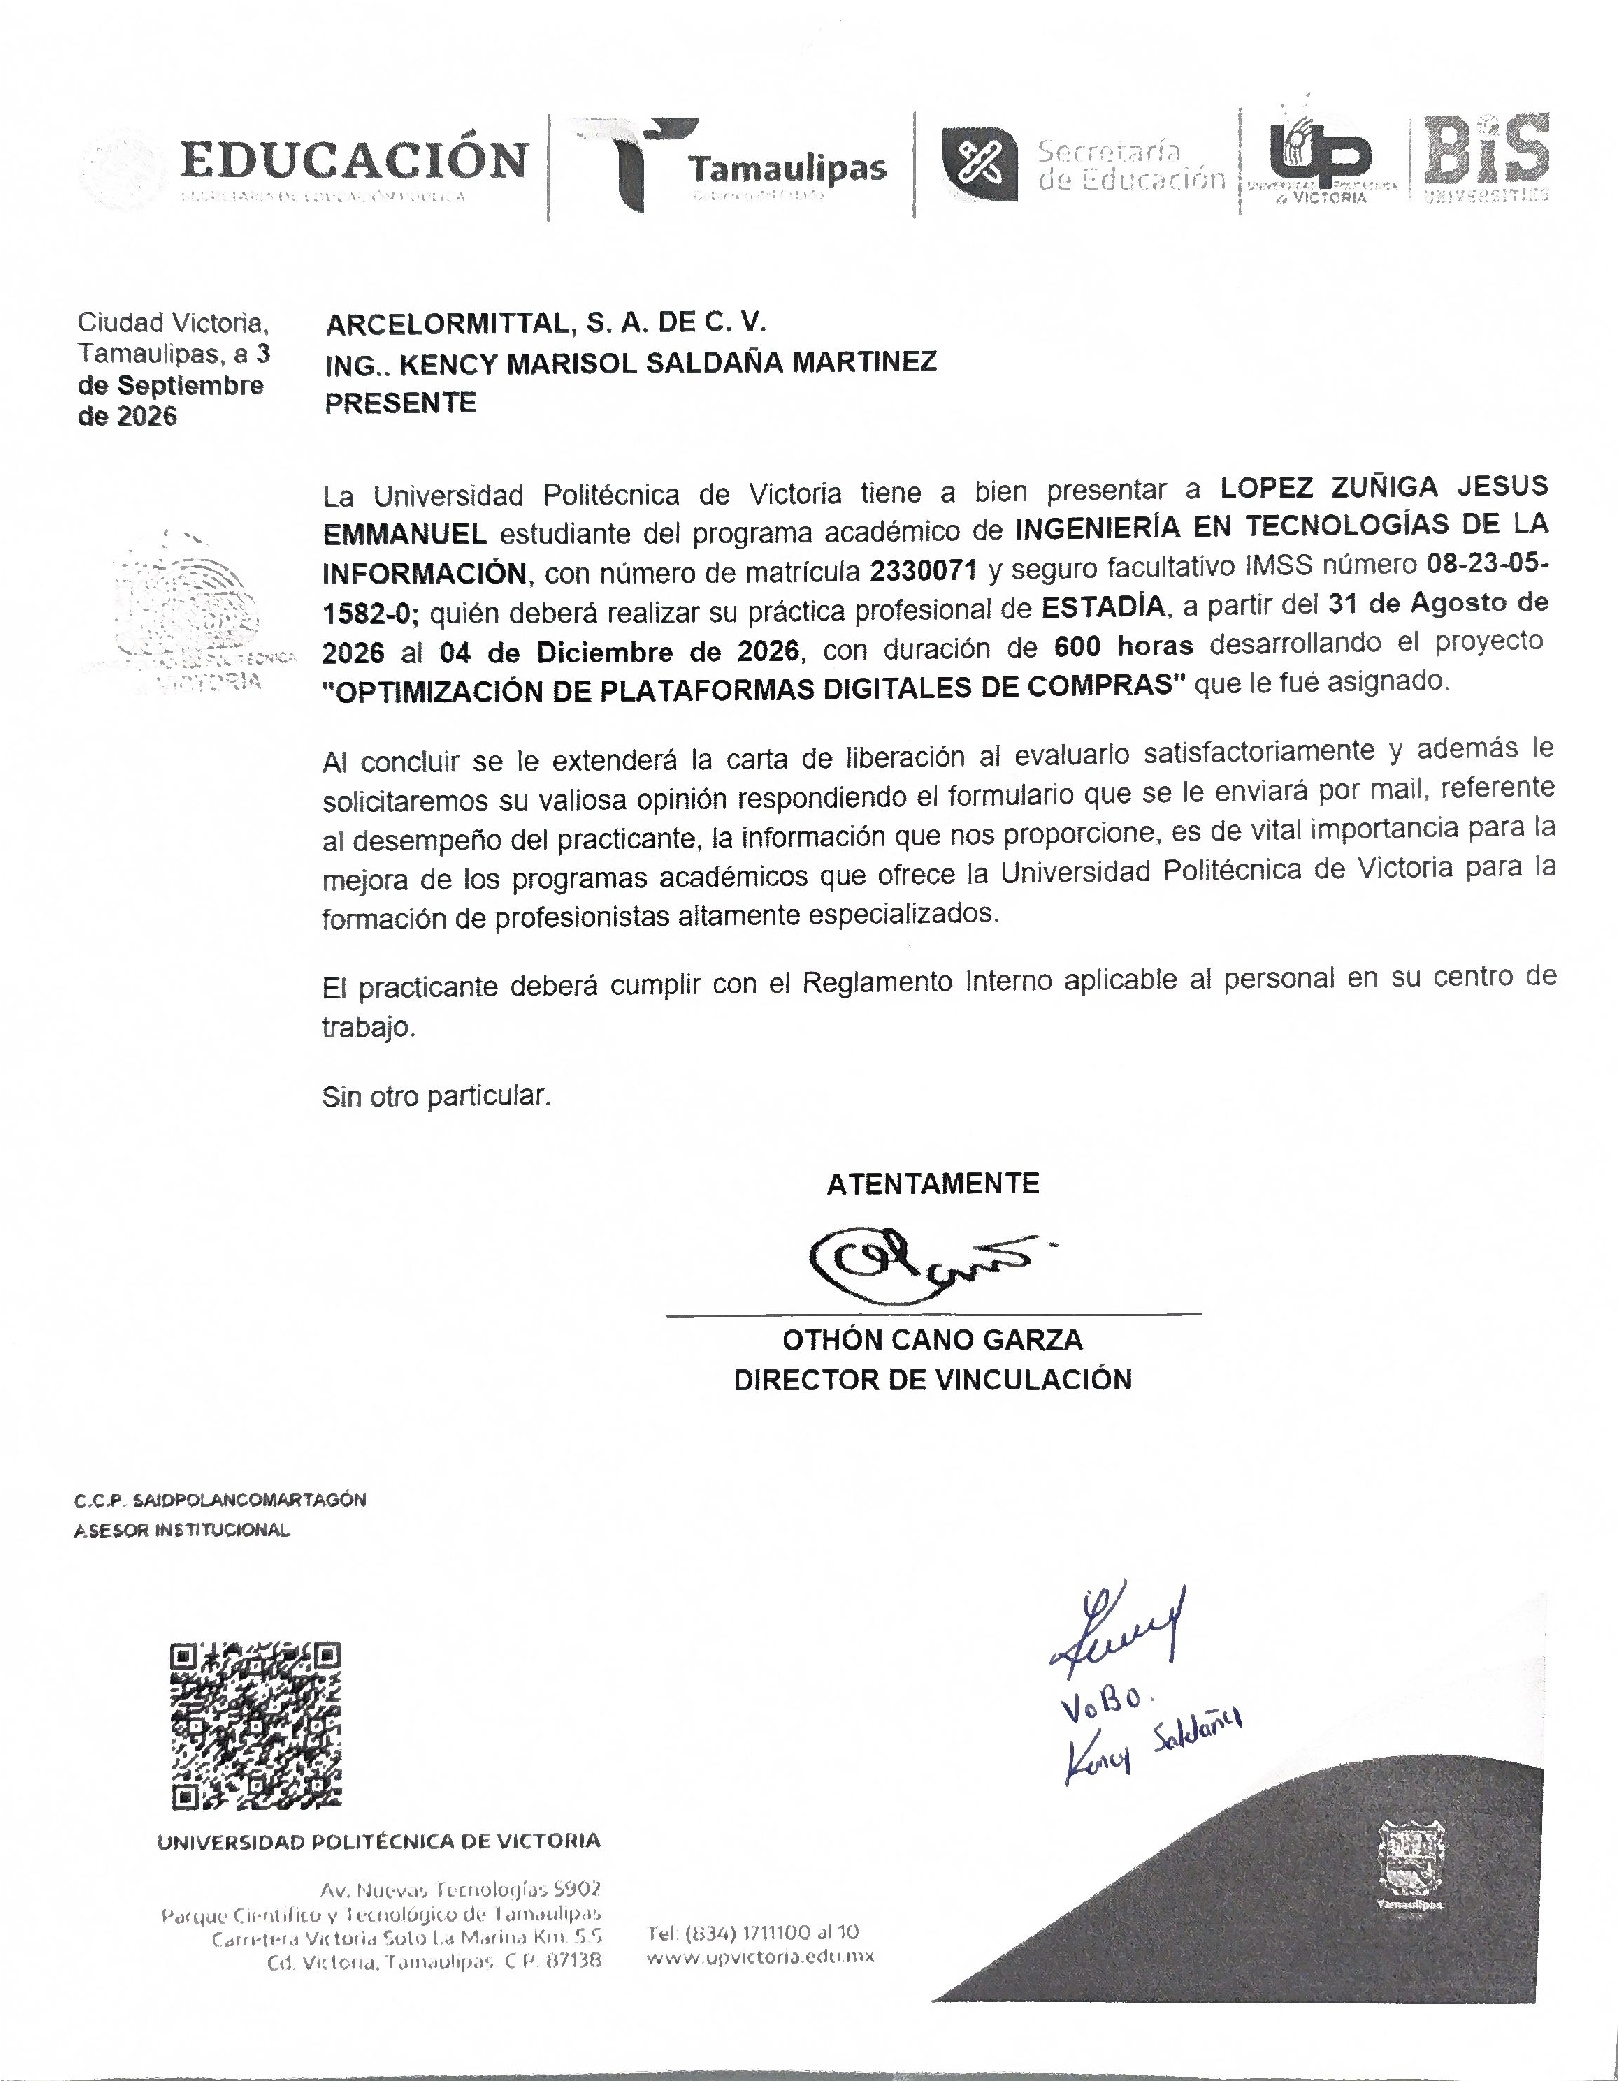
\includepdf[pages={1}]{cartas/CartaPresentacion.pdf}

% Pagina 2: Digitalización de la carta de aceptación (sustituir por una original en el empastado)
\clearpage
\thispagestyle{fancy}
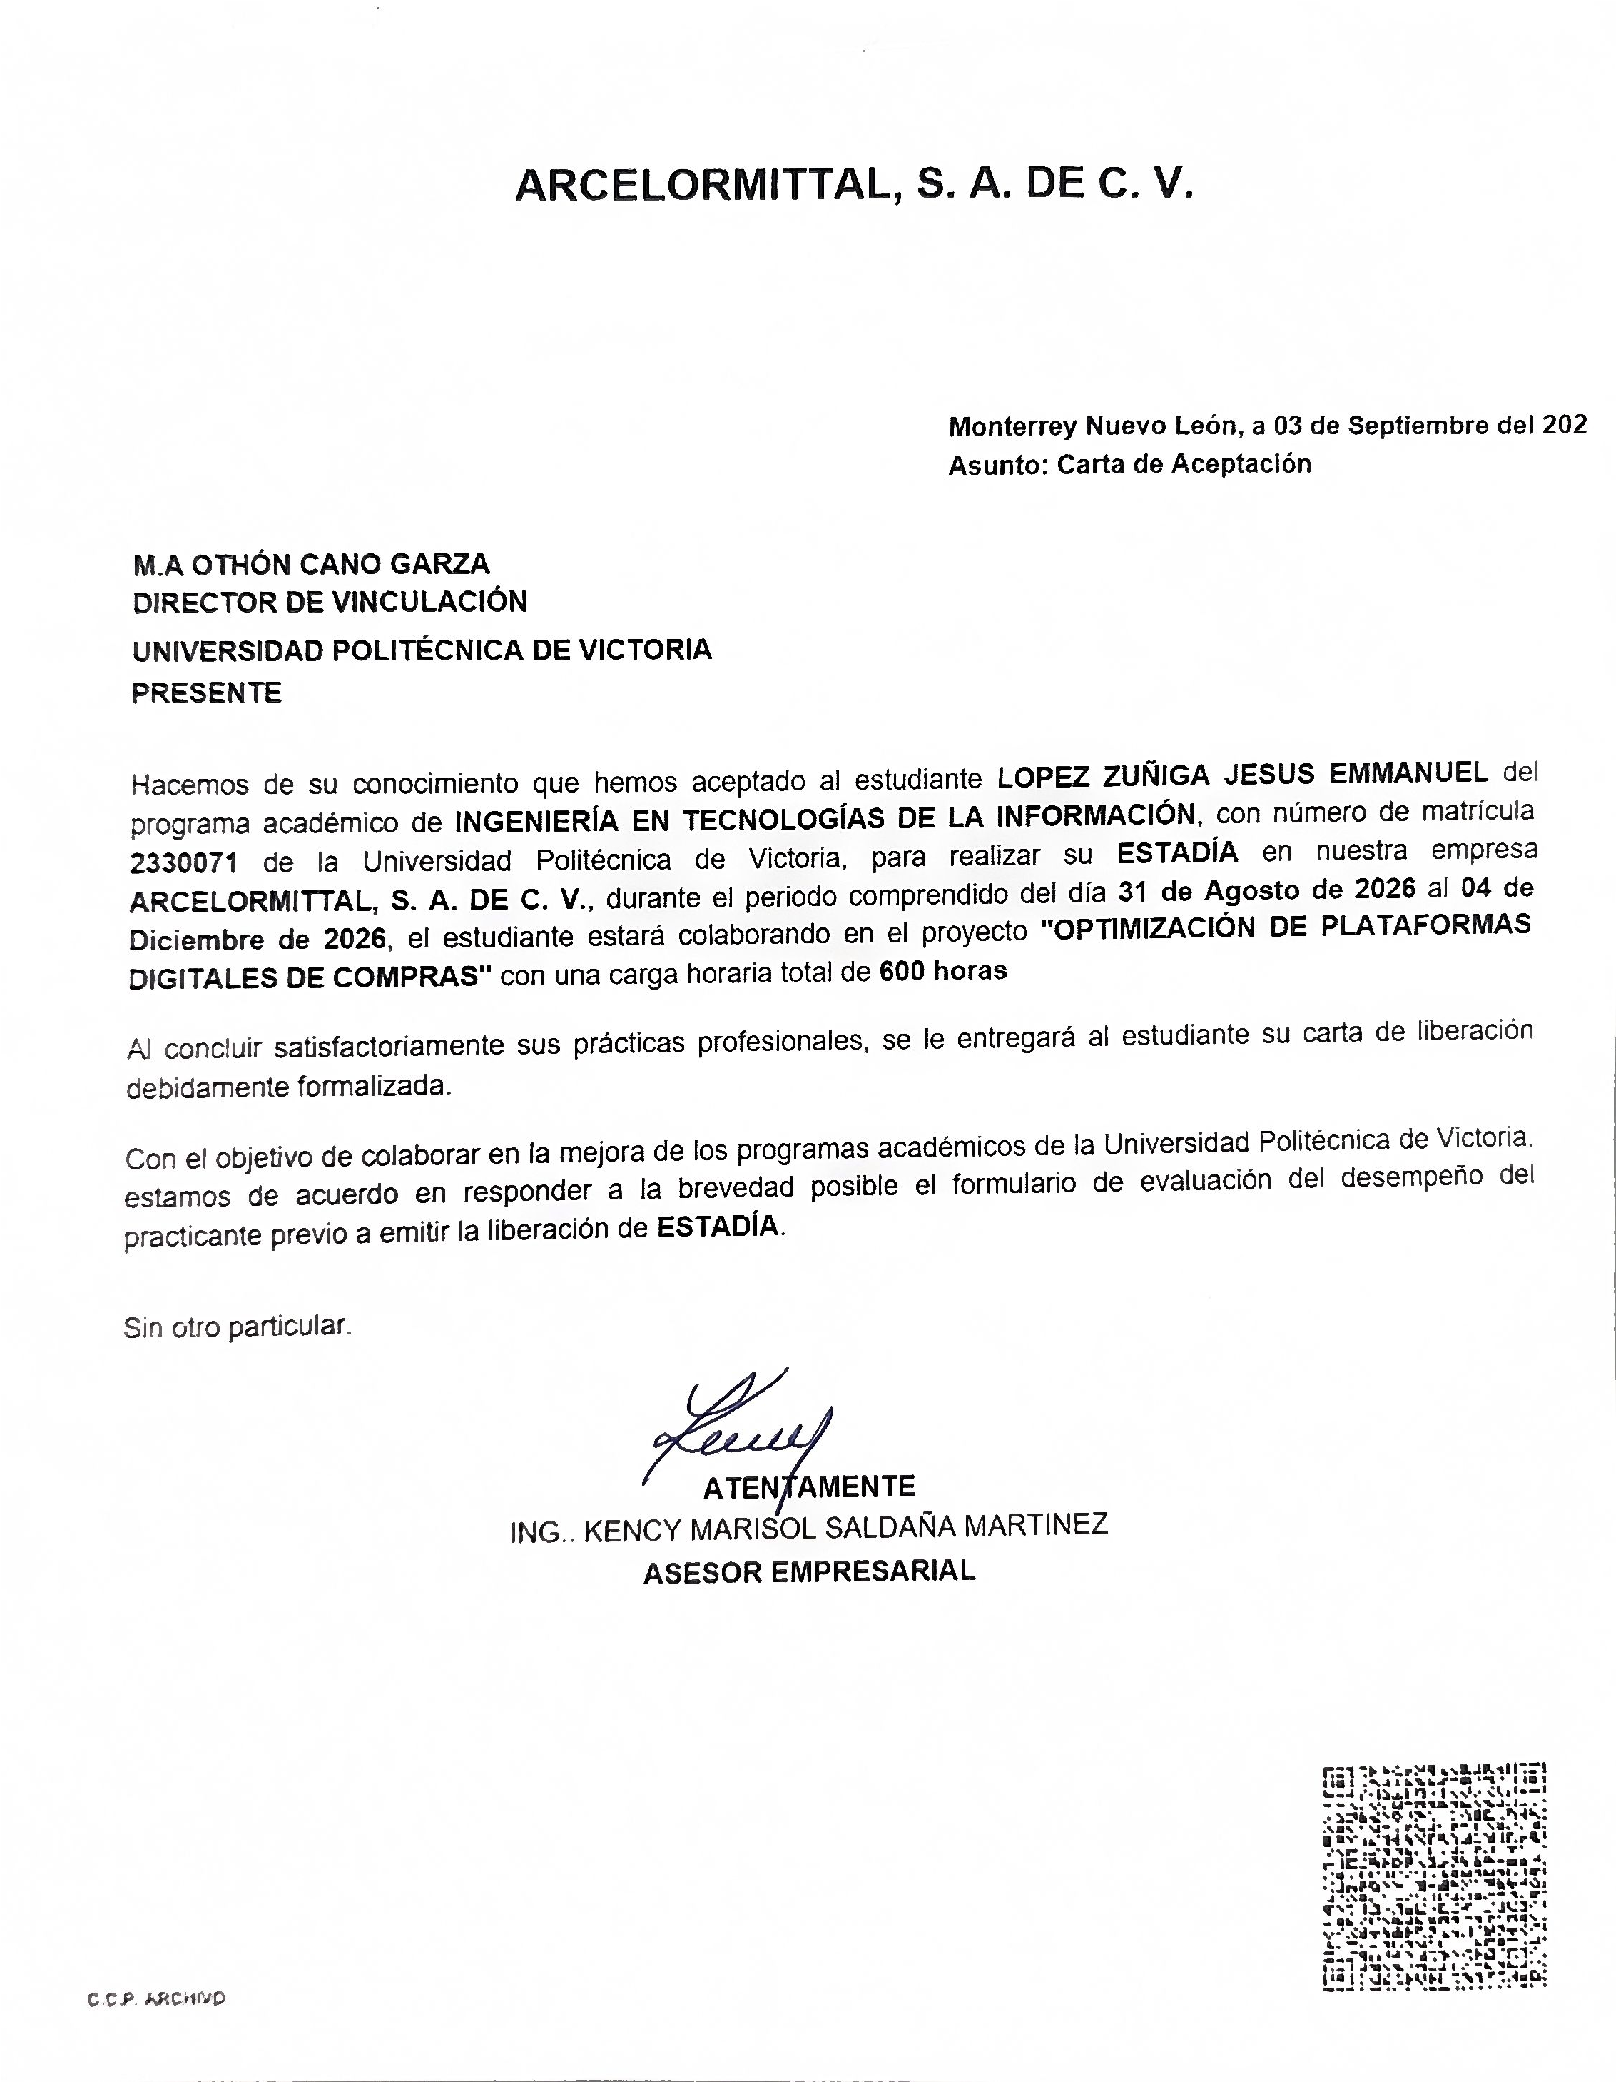
\includepdf[pages={1}]{cartas/CartaAceptacion.pdf}

% Pagina 3: Digitalización de la carta de liberación (sustituir por una original en el empastado)
\clearpage
\thispagestyle{fancy}
\includepdf[pages={1}]{cartas/CartaLiberacion.pdf}

% Pagina 4: Carta de aceptación del ASESOR INSTITUCIONAL(sustituir por una original en el empastado)
\clearpage
\ULCornerWallPaper{1}{membretes/membrete_UPV_08May25.pdf}
\thispagestyle{empty}

\vspace*{1.5cm}
\large

\begin{center}
\textbf{CARTA DE ACEPTACIÓN DEL DOCUMENTO PARA SU IMPRESIÓN}\\[\separacionLarga]
\end{center}

\begin{flushright}
Cd. Victoria, Tamaulipas a \fechacarta \\[\separacionLarga]
\end{flushright}

\parindent=0mm

\NombreAlumno \\
PRESENTE \\[\separacionCorta]

Le comunico que  el Programa Académico de \ncarrera\ \ le ha otorgado la autorización para la impresión de su Tesina de Estadía Práctica cuyo título es: \\[\separacionCorta]

\begin{center}
\textbf{\NombreProyecto} \\[\separacionLarga]
\end{center}

\begin{center}	
\begin{tabular}{ccc}
\centering
& ATENTAMENTE & \\ 
& & \\
& & \\
& & \\ \hline
& \nasesorinstitucional & \\
& ASESOR INSTITUCIONAL & \\
\end{tabular}
\end{center} 
\vspace{2cm}
c.c.p Director de programa académico

